\chapter{Теоретические сведения}

Цель работы --- получение навыков решения задачи Коши для ОДУ методами Пикара и явными методами первого порядка точности (Эйлера) и второго порядка точности (Рунге-Кутта).

\section{Входные данные}
Имеется ОДУ, не имеющее аналитического решения:
\begin{equation}
	\begin{cases}
		u'(x) = x^2 + u^2 \\
		u(0) = 0
	\end{cases}
\end{equation}

Необходимо найти значения функции $u(x)$ предложенными методами.

\section{Методы решения ОДУ}

Методы решения ОДУ можно разделить на:
\begin{itemize}
	\item точные;
	\item аналитически приближенные;
	\item численные.
\end{itemize} 
\subsection{Метод Пикара}
Относится к приближенным методам. Сводится к последовательному интегрированию полученного вида функции.
\begin{equation}
	y_s(x) = v_0 + \int_{x_0}^{x}\phi(t, y_{s -1}(t))dt, 
\end{equation}
где $y_s(x)$ – $s$-ое приближение искомой функции, $v_0 = y_0(t)$.
Тогда для заданного ОДУ приближения Пикара выглядят следующим образом:
Первое приближение:
\begin{equation}
	u_1(x) = 0 + \int_{0}^{x}t^2dt = \cfrac{x^3}{3}
\end{equation}

Второе приближение:
\begin{equation}
	u_2(x) = 0 + \int_{0}^{x}\left[t^2 + \left(\cfrac{t^3}{3}\right)^2\right] dt = \cfrac{x^3}{3} \cdot \cfrac{x^7}{9 \cdot 7}
\end{equation}
%
Третье приближение:
\begin{equation}
	\begin{array}{ll}
	u_3(x) = 0 + \int_{0}^{x}\left[ \left(\cfrac{t^7}{63} + \cfrac{t^3}{3} \right)^2 + t^2 \right] dt = 
	\int_{0}^{x}\left[ \cfrac{t^{14}}{63^2} + \cfrac{2}{63*3}t^{10} + \cfrac{t^6}{9} + t^2 \right] = \\
	\cfrac{x^3}{3} + \cfrac{x^7}{63} + \cfrac{2x^{11}}{2079} + \cfrac{x^{15}}{59535} 
	\end{array}
\end{equation}
%
Четвертое приближение:
\begin{equation}
	\begin{array}{ll}
	0 + \int_{0}^{x}\left[ \left( \cfrac{t^3}{3} + \cfrac{t^7}{63} + \cfrac{2t^{11}}{2079} +  \cfrac{t^{15}}{59535} \right)^2 + t^2 \right] dt = 
	\cfrac{x^3}{3} + \cfrac{x^{7}}{63} + \cfrac{2x^{11}}{2079} + \\+ \cfrac{13x^{15}}{218295} + \cfrac{82x^{19}}{37328445} +
	+ \cfrac{662x^{23}}{10438212015} + \cfrac{4x^{27}}{3341878155} + \cfrac{x^{31}}{109876903905}
	\end{array}
\end{equation}

\subsection{Метод Эйлера}
Относится к группе явных численных методов, имеет первый порядок точности. Общий вид поиска значения в следующем узле:
\begin{equation}
	y_{n + 1} = y_n + h \cdot f(x_n, y_n)
\end{equation}

где $f(x_n, y_n)$ --- функция, которой задано ОДУ, $h$ – шаг сетки для переменной $x$.

\subsection{Метод Рунге --- Кутта}
Vетод является численным и имеет второй порядок
точности. Вычисление значения в следующем узле выглядит следующим
образом:
\begin{equation}
	y_{n+1} = y_n + h*[(1-\alpha)k_1 + \alpha * k_2]
\end{equation}

Где $k_1$ и $k_2$ представлены как (\ref{eq:ref5}) и (\ref{eq:ref6}) соответственно, на практике $\alpha$ = 1 или $\cfrac{1}{2}$.

\begin{equation}
	k_1 = f(x_n, y_n)
	\label{eq:ref5}
\end{equation}

\begin{equation}
	k_2 = f(x_n + \cfrac{h}{2\alpha}, y_n + \cfrac{h}{2\alpha}k_1)
	\label{eq:ref6}
\end{equation}

\chapter{Программная реализация}
\captionsetup{singlelinecheck = false, justification=raggedright}
\begin{lstlisting}[label=lst:pcev,caption=Приближения для метода Пикара]
	func first_approx(x float64) float64 {
		return x * x * x / 3
	}
	
	func sec_approx(x float64) float64 {
		return first_approx(x) + math.Pow(x, 7)/63
	}
	
	func third_approx(x float64) float64 {
		return sec_approx(x) + 2*math.Pow(x, 11)/(3*7*9*11) + math.Pow(x, 15)/(9*9*7*7*15)
	}
	
	func fourth_approx(x float64) float64 {
		f := 4 * math.Pow(x, 15) / (3 * 3 * 7 * 9 * 11 * 15)
		s1 := 4 * math.Pow(x, 19) / (3 * 7 * 7 * 9 * 9 * 11 * 19)
		s2 := 2 * math.Pow(x, 19) / (3 * 9 * 9 * 7 * 7 * 15 * 19)
		t1 := 2 * math.Pow(x, 23) / (9 * 9 * 9 * 7 * 7 * 7 * 15 * 23)
		t2 := 2 * math.Pow(x, 23) / (3 * 3 * 7 * 7 * 9 * 9 * 11 * 11 * 23)
		fr := 4 * math.Pow(x, 27) / (3 * 7 * 7 * 7 * 9 * 9 * 9 * 11 * 15 * 27)
		fv := math.Pow(x, 31) / (9 * 9 * 9 * 9 * 7 * 7 * 7 * 7 * 15 * 15 * 31)
		
		return third_approx(x) + f + s1 + s2 + t1 + t2 + fr + fv
	}
\end{lstlisting}

\begin{lstlisting}[label=lst:pc,caption=Метод Пикара]
func PicardSolver(x0, h float64, n int) FloatMtx64 {
	values := MakeFloatMtx64(4, 0)
	
	for i := 0; i <= n; i++ {
		values[0] = append(values[0], first_approx(x0))
		values[1] = append(values[1], sec_approx(x0))
		values[2] = append(values[2], third_approx(x0))
		values[3] = append(values[3], fourth_approx(x0))
		
		x0 += h
	}
	return values
}
\end{lstlisting}

\begin{lstlisting}[label=lst:eu,caption=Метод Эйлера]
	func EulerSolver(x0, y0, h float64, n int) FloatVec64 {
		values := make(FloatVec64, 0)
		
		for i := 0; i <= n; i++ {
			values = append(values, y0)
			y0 += h * domain(x0, y0)
			x0 += h
		}
		
		return values
	}
\end{lstlisting}

\begin{lstlisting}[label=lst:rk,caption=Метод Рунге --- Кутта]
	func RungeKuttaSolver(x0, y0, alpha, h float64, n int) FloatVec64 {
		values := make(FloatVec64, 0)
		
		for i := 0; i <= n; i++ {
			values = append(values, y0)
			y0 += h * ((1-alpha)*domain(x0, y0) + alpha*domain(x0+h/2/alpha, y0+h*domain(x0, y0)/2/alpha))
			x0 += h
		}
		
		return values
	}
\end{lstlisting}

\begin{lstlisting}[label=lst:utils,caption=Вспомогательные функции и типы]
	type FloatVec64 []float64
	
	type FloatMtx64 []FloatVec64
	
	func MakeFloatMtx64(l, h int) FloatMtx64 {
		m := make(FloatMtx64, l)
		for i := 0; i < h; i++ {
			m[i] = make(FloatVec64, h)
		}
		return m
	}
	
	func domain(x, u float64) float64 {
		return x*x + u*u
	}
\end{lstlisting}

\chapter{Результаты расчетов}
\begin{table}[H]
	\captionsetup{singlelinecheck = false, justification=raggedleft}
	\renewcommand{\arraystretch}{1.8}
	\caption{Таблица результатов вычислений (начало)}
	\resizebox{\textwidth}{!}{
		\begin{tabular}{||c|c|c|c|c|c|c|c||}
			\hline
			№ & X & Пикар(1 пр.) & Пикар(2 пр.) & Пикар(3 пр.) & Пикар(4 пр.) & Эйлер & Рунге --- Кутт \\ \hline 
			1 & 0.00000 & 0.00000000 & 0.00000000 & 0.00000000 & 0.00000000  & 0.00000000   & 0.00000000   \\
			2 & 0.05000 & 0.00004167 & 0.00004167 & 0.00004167 & 0.00004167  & 0.00004154   & 0.00004167   \\
			3 & 0.10000 & 0.00033333 & 0.00033333 & 0.00033333 & 0.00033333  & 0.00033284   & 0.00033334   \\
			4 & 0.15000 & 0.00112500 & 0.00112503 & 0.00112503 & 0.00112503  & 0.00112390   & 0.00112503   \\
			5 & 0.20000 & 0.00266667 & 0.00266687 & 0.00266687 & 0.00266687  & 0.00266487   & 0.00266687   \\
			6 & 0.25000 & 0.00520833 & 0.00520930 & 0.00520930 & 0.00520930  & 0.00520618   & 0.00520930   \\
			7 & 0.30000 & 0.00900000 & 0.00900347 & 0.00900347 & 0.00900347  & 0.00899897   & 0.00900347   \\
			8 & 0.35000 & 0.01429167 & 0.01430188 & 0.01430189 & 0.01430189  & 0.01429574   & 0.01430189   \\
			9 & 0.40000 & 0.02133333 & 0.02135934 & 0.02135938 & 0.02135938  & 0.02135134   & 0.02135938   \\
			10 & 0.45000 & 0.03037500 & 0.03043431 & 0.03043446 & 0.03043446  & 0.03042424   & 0.03043446   \\
			11 & 0.50000 & 0.04166667 & 0.04179067 & 0.04179114 & 0.04179115  & 0.04177847   & 0.04179115   \\
			12 & 0.55000 & 0.05545833 & 0.05569999 & 0.05570133 & 0.05570134  & 0.05568590   & 0.05570134   \\
			13 & 0.60000 & 0.07200000 & 0.07244434 & 0.07244784 & 0.07244786  & 0.07242934   & 0.07244786   \\
			14 & 0.65000 & 0.09154167 & 0.09231980 & 0.09232824 & 0.09232831  & 0.09230633   & 0.09232831   \\
			15 & 0.70000 & 0.11433333 & 0.11564054 & 0.11565965 & 0.11565985  & 0.11563401   & 0.11565985   \\
			16 & 0.75000 & 0.14062500 & 0.14274379 & 0.14278465 & 0.14278523  & 0.14275505   & 0.14278524   \\
			17 & 0.80000 & 0.17066667 & 0.17399548 & 0.17407871 & 0.17408024  & 0.17404519   & 0.17408027   \\
			18 & 0.85000 & 0.20470833 & 0.20979686 & 0.20995931 & 0.20996315  & 0.20992261   & 0.20996322   \\
			19 & 0.90000 & 0.24300000 & 0.25059201 & 0.25089736 & 0.25090646  & 0.25085975   & 0.25090668   \\
			20 & 0.95000 & 0.28579167 & 0.29687639 & 0.29743135 & 0.29745200  & 0.29739841   & 0.29745263   \\
			21 & 1.00000 & 0.33333333 & 0.34920635 & 0.35018515 & 0.35023014  & 0.35016915   & 0.35023185   \\
			22 & 1.05000 & 0.38587500 & 0.40820993 & 0.40989019 & 0.40998477  & 0.40991653   & 0.40998919   \\
			23 & 1.10000 & 0.44366667 & 0.47459868 & 0.47741355 & 0.47760599  & 0.47753251   & 0.47761702   \\
			24 & 1.15000 & 0.50695833 & 0.54918087 & 0.55379315 & 0.55417345  & 0.55410128   & 0.55420008   \\
			25 & 1.20000 & 0.57600000 & 0.63287589 & 0.64028242 & 0.64101438  & 0.64096045   & 0.64107673   \\
			26 & 1.25000 & 0.65104167 & 0.72673010 & 0.73840666 & 0.73978212  & 0.73978624   & 0.73992422   \\
			27 & 1.30000 & 0.73233333 & 0.83193415 & 0.85003452 & 0.85256368  & 0.85271461   & 0.85288000   \\
			28 & 1.35000 & 0.82012500 & 0.94984168 & 0.97746847 & 0.98202821  & 0.98251740   & 0.98271806   \\ \hline
			
		\end{tabular}
	}
	\label{table:testing}
\end{table}

\begin{table}[H]
	\captionsetup{singlelinecheck = false, justification=raggedleft}
	\renewcommand{\arraystretch}{1.8}
	\caption{Таблица результатов вычислений (продолжение)}
	\resizebox{\textwidth}{!}{
		\begin{tabular}{||c|c|c|c|c|c|c|c||}
			\hline № & X & Пикар(1 пр.) & Пикар(2 пр.) & Пикар(3 пр.) & Пикар(4 пр.) & Эйлер & Рунге --- Кутт \\ \hline 
			29 & 1.40000 & 0.91466667 & 1.08198969 & 1.12355960 & 1.13163411  & 1.13286566   & 1.13311268   \\
			30 & 1.45000 & 1.01620833 & 1.23012049 & 1.29185290 & 1.30592042  & 1.30873502   & 1.30904442   \\
			31 & 1.50000 & 1.12500000 & 1.39620536 & 1.48677133 & 1.51092010  & 1.51705182   & 1.51744754   \\
			32 & 1.55000 & 1.24129167 & 1.58246992 & 1.71384867 & 1.75475104  & 1.76776607   & 1.76828516   \\
			33 & 1.60000 & 1.36533333 & 1.79142136 & 1.98002380 & 2.04846758  & 2.07572093   & 2.07642337   \\
			34 & 1.65000 & 1.49737500 & 2.02587752 & 2.29401209 & 2.40729662  & 2.46410778   & 2.46509613   \\
			35 & 1.70000 & 1.63766667 & 2.28899789 & 2.66677353 & 2.85244492  & 2.97133477   & 2.97279716   \\
			36 & 1.75000 & 1.78645833 & 2.58431668 & 3.11210160 & 3.41376070  & 3.66602195   & 3.66833681   \\
			37 & 1.80000 & 1.94400000 & 2.91577783 & 3.64736281 & 4.13368043  & 4.68409826   & 4.68813042   \\
			38 & 1.85000 & 2.11054167 & 3.28777229 & 4.29442366 & 5.07312176  & 6.33838527   & 6.34652466   \\
			39 & 1.90000 & 2.28633333 & 3.70517736 & 5.08080977 & 6.32033999  & 9.54566766   & 9.56699215   \\
			40 & 1.95000 & 2.47162500 & 4.17339840 & 6.04115248 & 8.00432170  & 18.64485062  & 18.74724488  \\
			41 & 2.00000 & 2.66666667 & 4.69841270 & 7.21898959 & 10.31515805 & 270.06840575 & 317.56647872 \\ \hline
	\end{tabular}}
\end{table}

\captionsetup{singlelinecheck = false, justification=centering}
\begin{center}
	\begin{figure}[H]
		\centering
		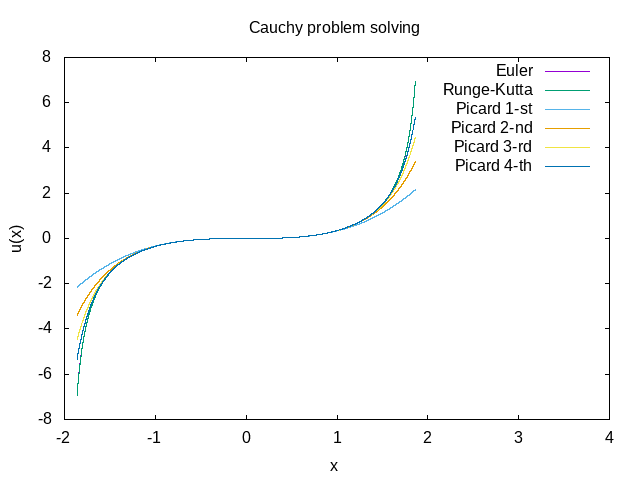
\includegraphics[width=0.9\linewidth]{assets/plot.png}
		\caption{График функции}
	\end{figure}
\end{center}

